\chapter{Markov propperty}
\section{Stochastic Parsing}
Stochastic parsing is the process of extracting syntactic structure of a given sentence based on 
statistical data from a given language. Such models in principle do not try to utilise any
semantic information in their analysis, but can aid semantic models by providing the parts of speech
a given word can be classified with in a given sentence. The ultimate goal of this project
is to create a universal stochastic parser which, based on implicitly assumed overarching
grammatical structure of human languages, could provide useful information about a completely
unknown language, by utilising statistical information from a set of known ones.
\subsubsection{Language specific tags}
Universal Dependencies framework allows for very fine grained representation of grammatical properties of a language,
to the point that certain categories exist only in a couple of available treebanks. More commonly, it allows for optional
specification of further information about a given role(eg. a noun's number or gender, which doesn't change its role in a sentence).
Since these additional classes do not change the grammatical structure of a sentence, and more importantly its graph, we've
decided to simply ignore them in our model. This means that our parser will not be able to tell that a noun is in its plural
form, or of a certain gender, but just that it is a noun. The purpose of this operation was to lower the number of parameters of our
model, there are 17 POS tags, and 37 syntactic relations, which is quite a lot, and further splitting it into subcategories might
mean that we won't have enough data to train our model.
\subsection{Hidden Markov Models(HMMs)}
We've thought very long on
how to approach this subject, as it is very complex, and we've never worked on anything related to NL processing. This was further
complicated by the fact that stochastic parsing is not often done in the context of UD. For a very long time at the beginning, we've been stuck thinking about how to
extract grammatical information from an arbitrary language, which proved to be very difficult, as languages transcribe grammatical information
in very different ways. Due to the difficulty of this task and the need to start writing an actual model, we've decided to abandon this line of approach.
Instead, we've realised that we can conclude weather a sentence has been correctly parsed without even knowing the language we're parsing, as long as we
are provided with its grammatical tree representation. So the first thought was to use a Bayesian network to analyse a sentence. Some further thinking revealed
regrettably, that this would require us to first check the probability of a sentence being of a given tree structure, and the number of those grows super exponentially
with the number of words in a sentence. We can however exploit the property, that each word in a correctly parsed UD dependency graph has only one parent node. This means, that there is only one path to the root, and that the probability of the parent node being classified in a certain way depends only on the probabilities of its children being in some states. This means, that for a specific path in a tree from a given node to the root, can be treated as a series of state changes, satisfying the Markov property. With this knowledge we've managed to find a lot of information about stochastic parsing, which ultimately allowed us to plan a general architecture of our parser. This key observation will be further elaborated upon in the next section.
\section{Proposed models}
A Markov model is a system of states with possibilities of transitions between them. They have been generalised to dynamic Bayesian networks, and in that form
they will be presented.
\begin{figure}[h!]
\center
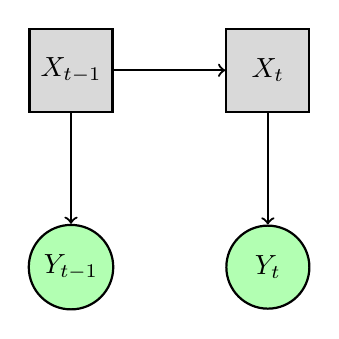
\begin{tikzpicture}[thick,node distance = {25mm},  state/.style = {draw, rectangle,fill= gray!30, minimum height=3em, minimum width=3em},
obs/.style = {draw, circle,fill= green!30, minimum height=3em, minimum width=3em}]
    
\node[state](1) {{$X_{t-1}$}};
    \node[state,right of=1](2) {{$X_t$}};
    \node[obs, below of=1](3) {{$Y_{t-1}$}};
    \node[obs, right of=3](4) {{$Y_{t}$}};
    \draw [->] (1) -- (2);
    \draw [->] (1) -- (3);
    \draw [->] (2) -- (4);
    
\end{tikzpicture}
\label{kal}
\caption{A Kalman filter described as a dynamic Bayesian network. The boxes represent the non observable state variables, and circles measurable data.}
\end{figure}

By exploiting the Markov property of the path from each node to the root of the tree, we can apply a Markov model of our choosing in analysing a whole sentence.
We will further exploit the fact that we can decide weather a sentence is parsed correctly only based on the tree produced, to split the model into two separate
parts. The first part will focus on analysing just the UD trees with a Markov model to produce the most probable parsings of a sentence. The other, which will for now depend heavily on the language under study, will give the probabilities for a word to be classified as a different part of speech based on its structure(for example, the english words ending with -ing can be either nouns or verbs). 


\clearpage
\subsection{Bare syntactic information}
For the purpose of analysing bare syntactic information, we propose Coupled Markov Model. This model we intuitively understand as most fittingly describing
the structure of the parse tree. We will assume that all states are observable, and that unconditional probabilities of all possible classifications are equal for both POS and syntactic relations. To train the model we will use sanitized datasets with language specific categories removed(which can be easily done in the CONLLu format). For now, we will only use data from one language(English) for training, but this can easily be extended to provide us with possible parse trees across hundreds of languages, and millions of sentences.
\begin{figure}[h!]
\center
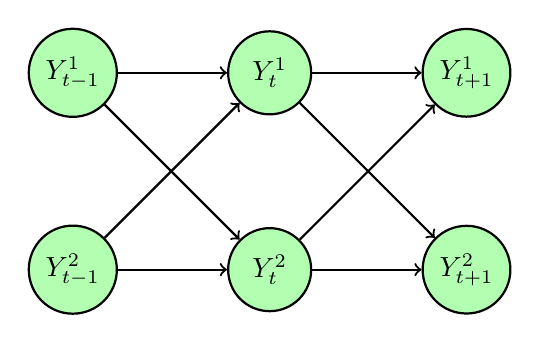
\begin{tikzpicture}[thick,node distance = {25mm},  state/.style = {draw, rectangle,fill= gray!30, minimum height=3em, minimum width=3em},
obs/.style = {draw, circle,fill= green!30, minimum height=3em, minimum width=3em}]
    
    \node[obs ](1) {{$Y_{t-1}^1$}};
    \node[obs, below of=1](2) {{$Y_{t-1}^2$}};

    \node[obs, right of=1](3) {{$Y_{t}^1$}};
    \node[obs, below of=3](4) {{$Y_{t}^2$}};

    \node[obs, right of=3](5) {{$Y_{t+1}^1$}};
    \node[obs, below of=5](6) {{$Y_{t+1}^2$}};


    \draw [->] (1) -- (3);
    \draw [->] (1) -- (4);

    \draw [->] (2) -- (3);
    \draw [->] (2) -- (4);
    
    \draw [->] (3) -- (5);
    \draw [->] (3) -- (6);

    \draw [->] (4) -- (5);
    \draw [->] (4) -- (6);
    
\end{tikzpicture}
\label{mark:synt}
\caption{Proposed complementary Markov model, with no hidden states representing the possible paths of a word to the root of the dependency tree}
\end{figure}
\subsection{Accounting for individual languages}
As mentioned before, we've had a lot of trouble in trying to find a universal way to extract grammatical information from a language. We are certain that
neural networks will be involved, but in order to use the training results across many languages, they have to be of a specific form. Since we aren't sure
what that form will be like, we will instead focus on interfacing with Markov Model. To this end, we propose a simple Recurrent neural network to classify
English words into its most probable POS tag and its syntactic relation to its head. This will require a lot of data, since there are a great many number of categories for each word, but since those are very regular, and we have a large dataset, we expect this task to not be very difficult. We can include it more directly
in our Markov model by having it provide us with an initial probability distribution for a given word.

\begin{figure}[h!]
\center
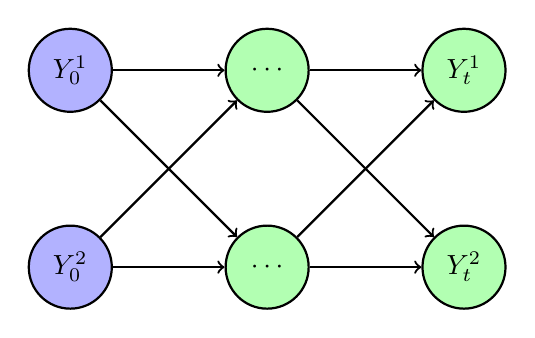
\begin{tikzpicture}[thick,node distance = {25mm},  state/.style = {draw, rectangle,fill= gray!30, minimum height=3em, minimum width=3em},
obs/.style = {draw, circle,fill= green!30, minimum height=3em, minimum width=3em}]
    
    \node[obs, fill=blue!30 ](1) {{$Y_{0}^1$}};
    \node[obs, fill=blue!30, below of=1](2) {{$Y_{0}^2$}};

    \node[obs, right of=1](3) {{$\cdots$}};
    \node[obs, below of=3](4) {{$\cdots$}};

    \node[obs, right of=3](5) {{$Y_{t}^1$}};
    \node[obs, below of=5](6) {{$Y_{t}^2$}};


    \draw [->] (1) -- (3);
    \draw [->] (1) -- (4);

    \draw [->] (2) -- (3);
    \draw [->] (2) -- (4);
    
    \draw [->] (3) -- (5);
    \draw [->] (3) -- (6);

    \draw [->] (4) -- (5);
    \draw [->] (4) -- (6);
    
\end{tikzpicture}
\label{mark:synt}
\caption{In this model, we assume that the initial probabilities for a given word(marked in blue), are provided by another model. This will change the probabilities of a word being tagged with a given POS tags, depending on the morphology of a word}
\end{figure}

One may think, that this breaks the Markov property, and in reality it does not, since we're using a Markov model only to generate possible paths to the root of the parse tree. The breaking of the Markov property will only occur once we try to combine those possible paths into a possible parse tree.
\clearpage

\subsection{Breakdown}
%    To summarize, the problem has been split into two separate problems. The first one being creating a language independent Markov model for UD parse trees. We assume that we can make it language independent by training it on parse trees from many different languages, which should train it to look for overarching grammatical structures across many different languages. One possible complication here, would be different sizes of tree banks. One could easily normalize circumvent this problem, by superimposing the Markov models over each other with different normalizing weights, but that issue will be dealt with once it appears.
%    The other being obtaining the initial probabilities. In training the model for obtaining these probabilities, we will assume that the only thing affecting them is the word itself, and not the other words in a sentence. We consider this a reasonable assumption, and expect those sentence wide relations to show up once combined with the Markov model. For the moment, this second problem will be interpreted as a simple classification problem, to be solved with a recurrent neural network. We will try to make the model as small as possible, and so will try to keep the network small.
%
To summarize, this chapter covered the use of the markov propperty between each node in the tree and its root in order to create a statistical "footprint" of a language. Since each language is different, each will have its own markov transition matrix that should produce the most likely paths through its syntax trees. Initialy, a word has a constant probability distribution in boths its classes. To create a more faithful model, these inital probabilities will be provided by a recurrent neural network described in the next chapter.
\subsubsection{Reality}
During implementation several issues turned up, which due to a lack of knowledge could not be remedied. The most important of which concerns the topology of the markov model. We've found no easily understood way to corelate the DEP and the POS transition matriecies in the split model, so a flattened model was used instead where each state is represented by a pair (POS,DEP).
This flattened model is very unwieldy, as it produces a sparse $666\times666$ matrix -- so sparse in fact that only 270 columns contain non--zero entries. It does however produce correct results, and even for large treebanks it can be calculated in a few minutes. This only has to be done once.
Regrettably however, despite the elegance of this approach, issues with the neural network precluded us from actualy putting it to use.


